% kuleuventheme2 by Janez Kren, September 2017, janez.kren@kuleuven.be, based on:
% kuleuventheme 1.3 by Roland Pastorino, 2013 roland.pastorino@kuleuven.be / www.rolandpastorino.com

\documentclass[10pt,t]{beamer}
\usetheme{kuleuven2}	%THEME OPTIONS for LOGO: kul (default), kulak, lrd,    ; OPTIONS for TITLE PAGE: normal (default), sedes


%%% OTHER SETTINGS
\usefonttheme[onlymath]{serif}			% math font with serifs, delete to make it sans-serif
\setbeamertemplate{footline}[body] 		% delete this line to remove footline bar on all frames
\usepackage[orientation=landscape,size=custom,width=16,height=9,scale=0.5,debug]{beamerposter} %enable for widescreen 16:9 ratio
%\titlegraphic{ \includegraphics[width=.2\paperwidth]{mytitlepagepic.png} } %optional title page image


%%% ADDED PACKAGES:
\usepackage[english]{babel}
\usepackage{amsfonts}
\usepackage{amssymb}
\usepackage{pgfplots}
\pgfplotsset{ticks=none}
\usepackage{xcolor}
\usepackage{graphicx}
\usepackage[export]{adjustbox}
\usepackage{cmbright}
\usepackage{csquotes}
\usepackage{minted}
\usemintedstyle{vs}
\usepackage[font=footnotesize]{caption}
\usepackage{subcaption}
\usepackage[capitalize]{cleveref}
\usepackage{xspace}
\usepackage{tabularx}
\usepackage{tablefootnote}
\usepackage{booktabs}
\usepackage{multirow}
\usepackage{array}
\usepackage{arydshln}

\usepackage{listofitems} % for \readlist to create arrays
\usetikzlibrary{arrows.meta} % for arrow size
\usepackage[outline]{contour} % glow around text
\contourlength{1.4pt}
\usetikzlibrary{decorations.markings}
\usetikzlibrary{backgrounds, calc, decorations.markings, intersections, mindmap, lindenmayersystems, snakes, through, trees}
\usepackage{pgf}
\usepackage{pgffor}
\usepgfmodule{shapes}
\usepgfmodule{plot}
\usetikzlibrary{decorations}
\usetikzlibrary{arrows}
\usetikzlibrary{snakes}
% \usetikzlibrary{external}
% \tikzexternalize[prefix=tikz/,optimize command away=\includepdf]

\usepackage{fontawesome}
\newcommand{\github}{GitHub~\faicon{github}}


\newcommand{\Gitter}[4]{
    \draw[very thin,color=gray] (#1,#3) grid (#2,#4);
}
\newcommand{\Koordinatenkreuz}[6]{
    \draw[->, >=latex, color=green!50!black] (#1,0) -- (#2,0) node[right] {#5};
    \draw[->, >=latex, color=green!50!black] (0,#3) -- (0,#4) node[left] {#6};
}
\newcommand{\KoordinatenkreuzOhneLabelsVerschobenKeinPfeil}[5]{
    \draw[-] (#1,0) -- (#2,0);
    \draw[-] (#5,#3) -- (#5,#4);

}
\newcommand{\latex}{\LaTeX}
\newcommand{\somespace}{\vskip.05\textheight}
\newcommand{\ZeigerdiagrammText}[4]{
\begin{tikzpicture}[scale=.72, samples=100, >=latex]

    \def\Alpha{#1}
    \def\Phase{#2}
    \def\AmplitudeSpannung{#3}
    \def\AmplitudeStrom{#4}
    \def\SpannungsWert{{\AmplitudeSpannung*sin(\Alpha)}}
    \def\StromWert{{\AmplitudeStrom*sin(\Alpha+\Phase)}}
    %%%%%%%%%%%%%%%%%%%%%%%%%%%%%%%%%%%%%%%%%%%%%%%%%%%%%%%%%%
    \def\FarbeSpannung{blue!90!white}
    \def\FarbeStrom{red!90!white}
    \def\FarbeWinkelZeichnung{green}
    %%%%%%%%%%%%%%%%%%%%%%%%%%%%%%%%%%%%%%%%%%%%%%%%%%%%%%%%%%
    \def\Beta{\Alpha+\Phase}
    \def\AlphaRad{\Alpha*3.141592654/180}
    \def\PhaseRad{\Phase*3.141592654/180}
    %%%%%%%%%%%%%%%%%%%%%%%%%%%%%%%%%%%%%%%%%%%%%%%%%%%%%%%%%%
    \Gitter{-.1}{7.1}{-3.1}{3.1}
    \Koordinatenkreuz{-.2}{7.3}{-3.2}{3.3}{$\omega t$}{}
    \draw (1.570795,0) node[below]{$\frac{\pi}{2}$};
    \draw (3.14159,0) node[below]{${\pi}$};
    \draw (4.71238898,0) node[below]{$\frac{3\pi}{2}$};
    \draw (6.283185307,0) node[below]{${2\pi}$};
    \draw (-4,0) circle (3cm);
    \KoordinatenkreuzOhneLabelsVerschobenKeinPfeil{-7.2}{-.8}{-3.6}{3.6}{-4}
    %%%%%%%%%%%%%%%%%%%%%%%%%%%%%%%%%%%%%%%%%%%%%%%%%%%%%%%%%%

    % voltage
    \draw[color=\FarbeSpannung, very thick] plot[id=voltage, domain=0:7] function{\AmplitudeSpannung*sin(x)} node[right] {$U(t)$};
    % voltage circle
    \draw[color=\FarbeSpannung, loosely dashed] (-4,0) circle (\AmplitudeSpannung cm);
    % angle
    \draw[color=\FarbeWinkelZeichnung!50!black, thick] (\AlphaRad, \SpannungsWert)--(\AlphaRad,\StromWert) node[below=18pt] {$\alpha$};
    % angle in the circle
    \filldraw[fill=\FarbeWinkelZeichnung!20,draw=\FarbeWinkelZeichnung!50!black] (-4,0) -- (-3,0) arc (0:\Alpha:1) -- cycle node[right] {$\alpha$};
    % voltage pointer
    \draw[<-,color=\FarbeSpannung, very thick] (\Alpha:\AmplitudeSpannung)++(-4,0) --(-4,0);
    \draw[color=\FarbeSpannung,  dashed] (\Alpha:\AmplitudeSpannung)++(-4,0) -- (\AlphaRad,\SpannungsWert);
    % current
    \draw[color=\FarbeStrom, very thick] plot[id=current, domain=0:7] function{\AmplitudeStrom*sin(x+\PhaseRad)} node[right] {$I(t)$};		
    % current circle
    \draw[color=\FarbeStrom, loosely dashed]    (-4,0) circle (\AmplitudeStrom cm);
    % current pointer
    \draw[<-,color=\FarbeStrom, very thick] (\Beta:\AmplitudeStrom)++(-4,0) --(-4,0);
    \draw[color=\FarbeStrom,  dashed](\Beta:\AmplitudeStrom)++(-4,0) -- (\AlphaRad,\StromWert);
    % phase difference
    \ifthenelse{\Phase<0}{
        \draw[snake=brace] (pi/2 ,3.3)--(pi/2-\PhaseRad ,3.3) node[above=7pt, left=10pt] {$\phi$};
    }
    {
        \draw[snake=brace] (pi/2-\PhaseRad ,3.3)--(pi/2 ,3.3) node[above=7pt, left=10pt] {$\phi$};
    }
    % angular velocity \omega
    \draw[->, xshift=-4cm]  (120:2.4cm) arc (120:170:2) node[below] {$\omega$};
\end{tikzpicture}
}

\colorlet{myred}{red!80!black}
\colorlet{myblue}{blue!80!black}
\colorlet{mygreen}{green!60!black}
\colorlet{myorange}{orange!70!red!60!black}
\colorlet{mydarkred}{red!30!black}
\colorlet{mydarkblue}{blue!40!black}
\colorlet{mydarkgreen}{green!30!black}

% STYLES
\tikzset{
  >=latex, % for default LaTeX arrow head
  node/.style={thick,circle,draw=myblue,minimum size=22,inner sep=0.5,outer sep=0.6},
  node in/.style={node,green!20!black,draw=mygreen!30!black,fill=mygreen!25},
  node hidden/.style={node,blue!20!black,draw=myblue!30!black,fill=myblue!20},
  node convol/.style={node,orange!20!black,draw=myorange!30!black,fill=myorange!20},
  node out/.style={node,red!20!black,draw=myred!30!black,fill=myred!20},
  connect/.style={thick,mydarkblue}, %,line cap=round
  connect arrow/.style={-{Latex[length=4,width=3.5]},thick,mydarkblue,shorten <=0.5,shorten >=1},
  node 1/.style={node in}, % node styles, numbered for easy mapping with \nstyle
  node 2/.style={node hidden},
  node 3/.style={node out}
}
\def\nstyle{int(\lay<\Nnodlen?min(2,\lay):3)} % map layer number onto 1, 2, or 3

\PassOptionsToPackage{hidelinks}{hyperref}
\usepackage{soul} % for \hl highlighting



\newcommand{\syntaxHighlight}[1]{\colorbox{black!10}{#1}}

%% to hide a column in table 
\usepackage{array}
\newcolumntype{H}{>{\setbox0=\hbox\bgroup}c<{\egroup}@{}}

\usepackage{booktabs}
\usepackage[dvipsnames,svgnames, table]{xcolor} % Required to specify custom colors
\usepackage[hidelinks]{hyperref} % hidelinks to remove ugly boxes
\usepackage{siunitx}
\DeclareSIUnit{\dBm}{dBm}	                % SI unit "dBm"
\DeclareSIUnit{\dBi}{dBi}                   % SI unit "dBi"
\DeclareSIUnit{\dBsm}{dBsm} 


\usepackage{pgfplots}
\usepgfplotslibrary{groupplots,dateplot}
\usetikzlibrary{patterns,shapes.arrows}
\usetikzlibrary{spy}
\pgfplotsset{compat=newest}
\usetikzlibrary{external}
\usetikzlibrary{calc}
\usetikzlibrary{shadings}
\usetikzlibrary{shadows.blur}
\usetikzlibrary{decorations.pathreplacing}

\usepackage{pgfplotstable}
% Enable external data files
\pgfplotsset{compat=1.18}

\usepackage{soul}

\input{auto_names}

\usepackage[xindy, nonumberlist]{glossaries}
\makenoidxglossaries%
%\makeglossaries%
\loadglsentries{abbr}%




\newcommand{\comm}[2]{\texttt{\textcolor{blue}{\textbackslash #1}\textcolor{red}{\{}#2\textcolor{red}{\}}}}
\newcommand{\commo}[1]{\texttt{\textcolor{blue}{\textbackslash #1}}}
\newcommand{\commop}[3]{\texttt{\textcolor{blue}{\textbackslash #1}[#2]\textcolor{red}{\{}#3\textcolor{red}{\}}}}
\newcommand{\pack}[1]{
        \texttt{\textcolor{magenta}{\textbackslash usepackage\{#1\}}}%
}
\newcommand{\commopt}[2]{
        \texttt{\textcolor{blue}{\textbackslash #1}}%
        \texttt{\textcolor{magenta}{\{#2\}}}%
}
\newcommand{\packopt}[2]{
        \texttt{\textcolor{magenta}{\textbackslash usepackage}}%
        \texttt{\textcolor{blue}{\lbrack #2\rbrack}}%
        \texttt{\textcolor{magenta}{\{#1\}}}%
}
\newcommand{\env}[3]{\texttt{\textcolor{olive}{\textbackslash begin\{#1\}}[#2]} \texttt{#3} \texttt{\textcolor{olive}{\textbackslash end\{#1\}}}}
\newcommand{\envt}[3]{\texttt{\textcolor{olive}{\textbackslash begin\{#1\}}\textcolor{red}{\{}#2\textcolor{red}{\}}} \texttt{#3} \texttt{\textcolor{olive}{\textbackslash end\{#1\}}}}
\newcommand{\envs}[2]{\texttt{\textcolor{olive}{\textbackslash begin\{#1\}}} \texttt{#2} \texttt{\textcolor{olive}{\textbackslash end\{#1\}}}}

\renewcommand{\emph}[1]{\textcolor{kul-blue}{#1}}
\newcommand{\Emph}[1]{\textcolor{kul-emph}{#1}}

\newcommand\TikZ{Ti\textit{k}Z\xspace}



%%% TITLE PAGE INFO:
\title[\LaTeX\ workshop]{\LaTeX\ workshop} %[]] will appear in footline
\subtitle{From novice to expert, to appreciator.} %Inspired by previous work from Dr.~Ing.~Jens Vankeirsbilck and Ing.\ Emanuele Peschiera

\author{Prof. Dr. Gilles Callebaut}
\institute{KU Leuven Ghent -- Dramco\\ \somespace \url{https://github.com/GillesC/LaTeX-Workshop}}
\date{}


\begin{document}
\defineauthors[false]{research, students}
\csname beamer@calculateheadfoot\endcsname %recalculate head and foot dimension

\small

\begin{frame}[plain,noframenumbering]
	\titlepage
\end{frame}


\begin{frame}[fragile]{References}
\begin{itemize}
    \item Thesis specific: \url{https://dramco edu.github.io/Thesis Tips-and-Tricks}
    \item Writing documents in \latex:  \url{https://github.com/DRAMCO/writing-scientific-papers-in-latex-tips-and-tricks}
    \item  \latex\ specific : \url{https://github.com/dramco-edu/LaTex}
    \item \latex\ Workshop: \url{https://github.com/GillesC/LaTeX-Workshop}
    \item Overleaf Documentation: \url{https://www.overleaf.com/learn}
\end{itemize}
\end{frame}

	

\section{Why \LaTeX?}
\begin{frame}[fragile,c]{Why LaTeX?}  %option fragile needed for verbatim environment

\begin{figure}
% 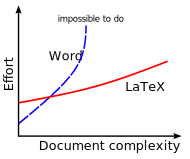
\includegraphics[scale=.3]{Figures/latex_vs_word}
\begin{tikzpicture}
    % Axis
    \draw[->, thick] (0,0) -- (7,0) node[midway, below] {Document complexity};
    \draw[->, thick] (0,0) -- (0,5) node[midway, above, rotate=90,anchor=south] {Effort};
    
    % Word curve: Starts slightly above origin, limited exponential growth
    \draw[blue, thick, dashed, domain=0:2.9] plot (\x, {0.5 + 0.3*\x*(\x+0.8)});
    \node[blue] at (3.4,4.2) {impossible to do};
    \node[blue] at (1.45,2.3) {Word};
    
    % LaTeX curve: Starts slightly above origin, linear to flattening
    \draw[red, thick, domain=0:6, smooth] plot (\x, {0.8 + 0.5*\x - 0.05*\x*\x});
    \node[red] at (2.8,1.2) {\LaTeX};

    \onslide<2->{\draw[red,fill=red] (0,0.8) circle (.5ex);}
    \onslide<2->{\draw[blue,fill=blue] (0,0.5) circle (.5ex);}
    \onslide<3->{\draw[red,fill=red] (2,0.8 + 0.5*2 - 0.05*2*2) circle (.5ex);}
    \onslide<3->{\draw[blue,fill=blue] (2,2.18) circle (.5ex);}
    \onslide<3->{ \draw [dashed] (2,0) -- (2,3);}

\end{tikzpicture}
\end{figure}
    
\end{frame}


\begin{frame}[fragile,c]{My goals for this workshop}
\begin{itemize}
    \item Express sympathy towards \LaTeX 
    \item Give an overview of the basics and elaborate on common pitfalls and must-have knowledge
    \item Provide a basis to fall back on (not everything will be covered in detail)
\end{itemize}
\end{frame}

\begin{frame}[fragile]{Things on how I am going to convince you to try \LaTeX}
\pause
\begin{itemize}[<+,10>]
    \item You can put text in comments and later retrieve old parts
    \item You can rearrange text easily by just switching some lines
    \item You can make unbelievably nice looking professional figures
    \item Using commands to replace words \research{}
    \item Abbreviations (and re-using them) \students{}
    \item Reusing the same colors in text, graphs to depict the same things \research{}
    \item Math in MS Word is awful.
    \item Referencing/citing becomes a worry of the past.
\end{itemize}
\end{frame}


% \begin{frame}[fragile]{Things on how I am going to convince you to try \LaTeX}
% \input{contents/example-colors}
% \end{frame}

\section{Getting up and running}
\begin{frame}[fragile]{Install LaTeX}

Distribution:
\begin{itemize}
	\item Tex Live for Windows (or MikTeX)
	\item TeX Live for Linux
	\item MacTeX for macOS
\end{itemize}
\vskip.05\textheight
Editors:
\begin{itemize}
	\item[] \Emph{VS Code}, \Emph{\href{https://www.overleaf.com/}{overleaf.com}}, TeXworks, TeXstudio, Texmaker, etc.
\end{itemize}
\end{frame}


\begin{frame}[fragile]{Using Overleaf}

Key features:
\begin{itemize}
	\item Setup-free \LaTeX 
	\item Visual Editor and Code Editor
	\item Project sharing
        \item \ldots
\end{itemize}
\vskip.05\textheight
Offline editors when:
\begin{itemize}
	\item Project is large (long compile time)
        \item More extensive features (e.g., with VS Code)
        \item Working offline
\end{itemize}
\end{frame}



\section{The basics}


\subsection{Starting a document}


% \begin{frame}[c,plain,noframenumbering]
% \begin{tikzpicture}[remember picture,overlay]
% \fill[fill=kul-blue]
%     (current page.south east)  rectangle  ([shift={(0,-0.1\paperheight)}]current page.north west)   ;
% \end{tikzpicture}

% \centering
% \vfill
% \textcolor{white}{\Large\textbf{Starting a document}}
% \end{frame}



\begin{frame}[fragile]{Starting a document}
Document class
\vspace{.5cm}
	\begin{columns}[t]
\begin{column}{.5\textwidth}
 \begin{minted}{latex}
    \documentclass{article}
    \begin{document}
        Hello world!
    \end{document}
 \end{minted}
\end{column}
		\begin{column}{.5\textwidth}
			\commo{documentclass} tells \latex\ how to lay out your document
			\vskip.05\textheight Standard classes are \Emph{article}, \Emph{report}, \Emph{book}, \Emph{letter}, \Emph{beamer} for presentations
			\vskip.05\textheight Each major publisher typically has its own class (e.g., IEEEtran)
		\end{column}
	\end{columns}	
\end{frame}

\begin{frame}[fragile]{Starting a document}
Preamble
\vspace{.5cm}
	\begin{columns}[t]
		\begin{column}{.5\textwidth}
			\texttt{\textcolor{blue}{\textbackslash documentclass}\textcolor{red}{\{}article\textcolor{red}{\}}
			\vskip.02\textheight
			\begin{tikzpicture}
			\filldraw [fill=orange!30, draw=orange] (5.5,1) rectangle (0,0);
			\end{tikzpicture}
			\\\textcolor{olive}{\textbackslash begin\{document\}}
			\\\quad Hello world!
			\\\textcolor{olive}{\textbackslash end\{document\}}
			}
		\end{column}
		\begin{column}{.5\textwidth}
			In the \textcolor{orange}{preamble}, you define which packages to use
			\begin{itemize}
				\item \packopt{babel}{english}
				\item \pack{graphicx}
			\end{itemize}
			\somespace
                \packopt{graphicx}{option1, option2}
            
		\end{column}
	\end{columns}	
\end{frame}


\begin{frame}[fragile]{Starting a document}
Document itself
\vspace{.5cm}
	\begin{columns}[t]
		\begin{column}{.5\textwidth}
			\texttt{\textcolor{blue}{\textbackslash documentclass}\textcolor{red}{\{}article\textcolor{red}{\}}
			\vskip.1\textheight
			\textcolor{olive}{\textbackslash begin\{document\}}
			\\\quad Hello world!
			\\\textcolor{olive}{\textbackslash end\{document\}}
			}
		\end{column}
		\begin{column}{.5\textwidth}
			\textcolor{olive}{\textbackslash begin\{...\}} and \textcolor{olive}{\textbackslash end\{...\}} define\\ the beginning and the ending\\ of an \textit{environment}
			\vskip.05\textheight \textcolor{olive}{\textbackslash begin\{document\}} and \textcolor{olive}{\textbackslash end\{document\}} identify where your document\\ starts and stops
		\end{column}
	\end{columns}	
\end{frame}


% \begin{frame}[fragile,c]{Goal of today}
% \textbf{Show you the basics}
% \begin{itemize}
% 	\item Starting a document
% 	\item Text structuring
% 	\item Figures, Tables, Equations, Algorithms and Listings
% 	\item Bibliography
% \end{itemize}	
% \vskip.05\textheight
% What if you need more than the basics?
% \vskip.05\textheight
% Try it yourself!
% \end{frame}


% \begin{frame}[c,plain,noframenumbering]
% \begin{tikzpicture}[remember picture,overlay]
% \fill[fill=kul-blue]
%     (current page.south east)  rectangle  ([shift={(0,-0.1\paperheight)}]current page.north west)   ;
% \end{tikzpicture}
% \centering
% \vfill
% \textcolor{white}{\Large\textbf{Text structuring}}
% \end{frame}


\begin{frame}[fragile]{Including a Title and an Author}
\vspace{.5cm}
	\begin{columns}[t]
		\begin{column}{.5\textwidth}
			\texttt{\textcolor{blue}{\textbackslash documentclass}\textcolor{red}{\{}article\textcolor{red}{\}}
			\\\comm{title}{My First Document}
			\\\comm{author}{E. Peschiera}
			\\\comm{date}{}
			\\\textcolor{olive}{\textbackslash begin\{document\}}
			\\\quad\commo{maketitle}
			\\\quad Hello world!
			\\\textcolor{olive}{\textbackslash end\{document\}}
			}
		\end{column}
		\begin{column}{.5\textwidth}
			\comm{title}{...} and \comm{author}{...} \\are self-explanatory
			\vskip.05\textheight \comm{date}{} is useful to suppress the\\ showing of the current date
			\vskip.05\textheight \commo{maketitle} is fundamental! Without it,\\ title and author are excluded
		\end{column}
	\end{columns}	
    \somespace
    \somespace
    \begin{center}
        \Emph{Note: templates can define their own title/author commands.}
    \end{center}
\end{frame}

\begin{frame}[fragile]{Including a Title and an Author}
Result
\vspace{.5cm}
	\begin{columns}[t]
		\begin{column}{.5\textwidth}
			\texttt{\textcolor{blue}{\textbackslash documentclass}\textcolor{red}{\{}article\textcolor{red}{\}}
			\\\comm{title}{My First Document}
			\\\comm{author}{G. Callebaut}
			\\\comm{date}{}
			\\\textcolor{olive}{\textbackslash begin\{document\}}
			\\\quad\commo{maketitle}
			\\\quad Hello world!
			\\\textcolor{olive}{\textbackslash end\{document\}}
			}
		\end{column}
		\begin{column}{.5\textwidth}
			\begin{figure}
			\includegraphics[width=.9\linewidth, frame, trim={-1cm -1cm -1cm -1cm},clip]{Figures/doc1}
			\end{figure}
		\end{column}
	\end{columns}	
\end{frame}

\begin{frame}[fragile]{Including Structuring Elements}
\vspace{.5cm}
	\begin{columns}[t]
		\begin{column}{.5\textwidth}
			Numbered elements
			\begin{itemize}
				\item \comm{chapter}{...}
				\item \comm{section}{...}
				\item \comm{subsection}{...}
				\item \comm{subsubsection}{...}
			\end{itemize}
			Unnumbered elements, same commands \\but with *
			\begin{itemize}
				\item \comm{chapter\textsuperscript{\textcolor{black}{*}}}{...}
			\end{itemize}
		\end{column}
		\begin{column}{.5\textwidth}
			Depending on the template, certain elements might not be present
			\begin{itemize}
				\item \comm{chapter}{} only in books and reports
				\item No structuring elements\\ supported in letters
			\end{itemize}
		\end{column}
	\end{columns}	
\end{frame}

\begin{frame}[fragile]{Including Structuring Elements}
%\vspace{.5cm}
	\begin{columns}[t]
		\begin{column}{.5\textwidth}
			\begin{figure}
			\includegraphics[scale=.5]{Figures/code1}
			\end{figure}
		\end{column}
		\begin{column}{.5\textwidth}
			\begin{figure}
			\includegraphics[width=.79\linewidth, frame, trim={-1cm -1cm -1cm -1cm},clip]{Figures/doc2}
			\end{figure}
		\end{column}
	\end{columns}	
\end{frame}

\subsection{Figures and Tables}
% \begin{frame}[c,plain,noframenumbering]
% \begin{tikzpicture}[remember picture,overlay]
% \fill[fill=kul-blue]
%     (current page.south east)  rectangle  ([shift={(0,-0.1\paperheight)}]current page.north west)   ;
% \end{tikzpicture}
% \centering
% \vfill
% \textcolor{white}{\Large\textbf{Figures, Tables, Equations, \\\vspace{0.3cm}Algorithms and Listings}}
% \end{frame}

% \begin{frame}[c,plain,noframenumbering]
% \begin{tikzpicture}[remember picture,overlay]
% \fill[fill=gray]
%     (current page.south east)  rectangle ([shift={(0,-0.1\paperheight)}]current page.north west)   ;
% \end{tikzpicture}
% \centering
% \vfill
% \textcolor{white}{\Large\textbf{Figures}}
% \end{frame}


\begin{frame}[fragile]{Including a Figure}
\vspace{.5cm}
	\begin{columns}[t]
		\begin{column}{.5\textwidth}
			Need graphicx package
			\\\quad \pack{graphicx}
			\vskip.05\textheight
			Define a figure environment
			\begin{itemize}
			\item[] \env{figure}{placing specifier}{
			\\\quad \commo{centering}
			\\\quad \commop{includegraphics}{options}{\\pathToFigure}
			\\\quad \comm{caption}{text explaining\\ the figure}\\
			}
			\end{itemize}
		\end{column}
		\begin{column}{.5\textwidth}
			[placing specifier]
			\begin{itemize}
				\item h = here
				\item t = top of the page
				\item b = bottom of the page
				\item p = on a special page for \textit{figures}, \textit{tables}, \textit{etc.}
				\item ! = override LaTeX parameters that normally decide good positioning
			\end{itemize}
		\end{column}
	\end{columns}	
\end{frame}

\begin{frame}[fragile]{Including a Figure}
\vspace{.5cm}
	\begin{columns}[t]
		\begin{column}{.5\textwidth}
			Need graphicx package
			\\\quad \pack{graphicx}
			\vskip.05\textheight
			Define a figure environment
			\begin{itemize}
			\item[] \env{figure}{placing specifier}{
			\\\quad \commo{centering}
			\\\quad \commop{includegraphics}{options}{\\pathToFigure}
			\\\quad \comm{caption}{text explaining\\ the figure}\\
			}
			\end{itemize}
		\end{column}
		\begin{column}{.5\textwidth}
			\commo{centering} makes sure the included figure is centered in the environment
			\vskip.05\textheight
			similar placing as in figures, but now with respect to the other subfigures.
		\end{column}
	\end{columns}	
\end{frame}

\begin{frame}[fragile]{Using Subfigures}
\vspace{.5cm}
	\begin{columns}[t]
		\begin{column}{.5\textwidth}
			Needs
			\\\quad \pack{caption}
                \\\quad \pack{subcaption}
			\vskip.05\textheight
			Define a figure environment
			\begin{itemize}
			\item[] \env{figure}{placing specifier}{
                \\ \quad \env{subfigure}{placing specifier}{
                \\\qquad \commo{includegrpahics}}\\
                \commo{hfill}
                 \\ \quad \env{subfigure}{placing specifier}{
                \\}\\
			}\\
			\end{itemize}
		\end{column}
		\begin{column}{.5\textwidth}
			\commo{subfigure} allows to place different subfigures in one figure environment.
			\vskip.05\textheight
			\commo{includegraphics} finds and inserts the actual figure file
			\begin{itemize}
				\item optional typically refers to the \\width or height of the figure
				\item most often related to \commo{textwidth}, e.g. \texttt{[width=0.5\commo{textwidth}]}
			\end{itemize}
		\end{column}
	\end{columns}	
\end{frame}

% \begin{frame}[fragile]{Including a Figure}
% %\vspace{.5cm}
% 	\begin{columns}[t]
% 		\begin{column}{.5\textwidth}
% 			\begin{figure}
% 			\includegraphics[scale=.45]{Figures/code2}
% 			\end{figure}
% 		\end{column}
% 		\begin{column}{.5\textwidth}
% 			\begin{figure}
% 			\includegraphics[width=.72\linewidth, frame, trim={-1cm -1cm -1cm -1cm},clip]{Figures/doc3}
% 			\end{figure}
% 		\end{column}
% 	\end{columns}	
% \end{frame}

% \begin{frame}[c,plain,noframenumbering]
% \begin{tikzpicture}[remember picture,overlay]
% \fill[fill=gray]
%     (current page.south east)  rectangle ([shift={(0,-0.1\paperheight)}]current page.north west)   ;
% \end{tikzpicture}
% \centering
% \vfill
% \textcolor{white}{\Large\textbf{Tables}}
% \end{frame}

\begin{frame}[fragile]{Inserting a Table}
\vspace{.5cm}
	\begin{columns}[t]
		\begin{column}{.5\textwidth}
			\env{table}{placing options}{\begin{itemize}
			\item[] \comm{caption}{text explaining the Table}
			\\ \commo{centering}
			\envt{tabular}{columnFormat}{
			\\\quad colTitle \textcolor{red}{\&} \textless repeat for all columns\textgreater \textcolor{blue}{ \textbackslash\textbackslash}
			\\\quad \commo{hline}
			\\\quad data \textcolor{red}{\&} data \textcolor{red}{\&} \textless repeat\textgreater   \textcolor{blue}{ \textbackslash\textbackslash}
			\\\quad \commo{hline}\\}
			\end{itemize}
			}
		\end{column}
		\begin{column}{.5\textwidth}
			\texttt{\textcolor{olive}{table}} environment makes sure that\\ the table can be correctly placed
			\vskip.05\textheight
			\texttt{\textcolor{olive}{tabular}} environment \\= actual table
		\end{column}
	\end{columns}	
\end{frame}

\begin{frame}[fragile]{Inserting a Table}
\vspace{.5cm}
	\begin{columns}[t]
		\begin{column}{.5\textwidth}
			\env{table}{placing options}{\begin{itemize}
			\item[] \comm{caption}{text explaining the Table}
			\\ \commo{centering}
			\envt{tabular}{columnFormat}{
			\\\quad colTitle \textcolor{red}{\&} \textless repeat for all columns\textgreater \textcolor{blue}{ \textbackslash\textbackslash}
			\\\quad \commo{hline}
			\\\quad data \textcolor{red}{\&} data \textcolor{red}{\&} \textless repeat\textgreater   \textcolor{blue}{ \textbackslash\textbackslash}
			\\\quad \commo{hline}\\}
			\end{itemize}
			}
		\end{column}
		\begin{column}{.5\textwidth}
			\texttt{\textcolor{red}{\{}columnFormat\textcolor{red}{\}}} defines
			\begin{itemize}
				\item How many columns in the table
				\item The layout of the columns
				\begin{itemize}
					\item c: centered text
					\item l: left-aligned text
					\item r: right-aligned text
                        \item fixed-width columns \texttt{p\{2cm\}}
                        \begin{itemize}
                            \item m: middle
                            \item p: top
                            \item b: bottom
                        \end{itemize}
				\end{itemize}
				% \item When to draw vertical lines, defined by \textbar
			\end{itemize}
		\end{column}
	\end{columns}	
\end{frame}

\begin{frame}[fragile]{Inserting a Table}
\vspace{.5cm}
	\begin{columns}[t]
		\begin{column}{.5\textwidth}
			\env{table}{placing options}{
			\begin{itemize}
			\item[] \comm{caption}{text explaining the Table}
			\\ \commo{centering}
			\envt{tabular}{columnFormat}{
			\\\quad colTitle \textcolor{red}{\&} \textless repeat for all columns\textgreater \textcolor{blue}{ \textbackslash\textbackslash}
			\\\quad \commo{hline}
			\\\quad data \textcolor{red}{\&} data \textcolor{red}{\&} \textless repeat\textgreater   \textcolor{blue}{ \textbackslash\textbackslash}
			\\\quad \commo{hline}\\}
			\end{itemize}
			}
		\end{column}
		\begin{column}{.5\textwidth}
			\texttt{\textcolor{red}{\&}} is a column separator. Used to show in which column the next \textit{item} goes
			\vskip.05\textheight
			\commo{hline} inserts a horizontal line
			\vskip.05\textheight
			\commo{\textbackslash} is the standard LaTeX command for\\ a line break
			\\\quad In a table: next row
		\end{column}
	\end{columns}	
\end{frame}

\begin{frame}[fragile]{Inserting a Table}
%\vspace{.5cm}
	\begin{columns}[t]
		\begin{column}{.5\textwidth}
			\begin{figure}
			\includegraphics[scale=.35]{Figures/code3}
			\end{figure}
		\end{column}
		\begin{column}{.5\textwidth}
			\begin{figure}
			\includegraphics[width=.85\linewidth, frame, trim={-1cm -1cm -1cm -1cm},clip]{Figures/doc4}
			\end{figure}
		\end{column}
	\end{columns}	
\end{frame}

\begin{frame}[fragile]{Note on Figures and Tables}
\vspace{.5cm}
	In case your document is multicolumn, e.g., IEEE paper, but your figure needs to\\ span more than 1 column:
	use * when defining the environment
	\vskip.02\textheight
	\begin{itemize}
		\item[] \envs{figure*}{...}
%		\vskip.01\textheight
		\item[] \envs{table*}{...}
	\end{itemize}
\end{frame}


\begin{frame}[fragile]{Making beautiful tables}
	Highly recommended document: \url{https://people.inf.ethz.ch/markusp/teaching/guides/guide-tables.pdf}.
	\somespace
    Guidelines
	\begin{itemize}
		\item avoid vertical lines
        \item Avoid “boxing up” cells, usually 3 horizontal lines are
enough: above, below, and after heading (see examples in
this guide)
\item avoid double horizontal lines
\item enough space between rows
\item if in doubt, align left
\item right-align numbers (using same notation/unit)
        \item use \pack{booktabs}
	\end{itemize}
\end{frame}


\begin{frame}[fragile]{Making beautiful tables}

\newcommand{\ra}[1]{\renewcommand{\arraystretch}{#1}}
\centering
\resizebox{0.9\textwidth}{!}{%
\ra{1.3}
\setlength\dashlinedash{0.2pt}
\setlength\dashlinegap{1.5pt}
\setlength\arrayrulewidth{0.3pt}

% \begin{tabular}{@{}rrrrcrrrcrrr@{}}\toprule
% & \multicolumn{3}{c}{$w = 8$} & \phantom{abc}& \multicolumn{3}{c}{$w = 16$} &
% \phantom{abc} & \multicolumn{3}{c}{$w = 32$}\\
% \cmidrule{2-4} \cmidrule{6-8} \cmidrule{10-12}
% & $t=0$ & $t=1$ & $t=2$ && $t=0$ & $t=1$ & $t=2$ && $t=0$ & $t=1$ & $t=2$\\ \midrule
% $dir=1$\\
% $c$ & 0.0790 & 0.1692 & 0.2945 && 0.3670 & 0.7187 & 3.1815 && -1.0032 & -1.7104 & -21.7969\\
% $c$ & -0.8651& 50.0476& 5.9384&& -9.0714& 297.0923& 46.2143&& 4.3590& 34.5809& 76.9167\\
% $c$ & 124.2756& -50.9612& -14.2721&& 128.2265& -630.5455& -381.0930&& -121.0518& -137.1210& -220.2500\\
% $dir=0$\\
% $c$ & 0.0357& 1.2473& 0.2119&& 0.3593& -0.2755& 2.1764&& -1.2998& -3.8202& -1.2784\\
% $c$ & -17.9048& -37.1111& 8.8591&& -30.7381& -9.5952& -3.0000&& -11.1631& -5.7108& -15.6728\\
% $c$ & 105.5518& 232.1160& -94.7351&& 100.2497& 141.2778& -259.7326&& 52.5745& 10.1098& -140.2130\\
% \bottomrule
% \end{tabular}

\begin{tabular}{@{}lllrrr@{}}\toprule
\textbf{Rank} & \textbf{Lead Arranger} & \textbf{Number of Deals} & \textbf{Dollar Amount} & \textbf{Market Share} & \textbf{Equator Principles Adoption}\\ \midrule
\textbf{1} & State Bank of India & 52 & \$21,631.6 & 10.1\% & NA\\ \hdashline
\textbf{2} & Mitsubishi UFJ Financial & 88 & 9,486.1 & 4.4 & Dec 2005\\ \hdashline
\textbf{3} & Sumitomo Mitsui & 71 & 8,188.1 & 3.8 & Jan 2006\\ \hdashline
\textbf{4} & Credit Agrocole & 60 & 6,506.4 & 3.1 & Jun 2005\\ \hdashline
\textbf{5} & Mizuho Financial & 55 & 5,797.5 & 2.7 & Oct 2003\\ \hdashline
\textbf{6} & Soci\'{e}t\'{e} Generale & 55 & 5,760.5 & 2.7 & Sep 2007\\ \hdashline
\textbf{7} & BNP Paribas & 55 & 5,390.8 & 2.5 & Oct 2008\\ \hdashline
\textbf{8} & Axis Bank & 18 & 5,216.9 & 2.4 & NA\\ \hdashline
\textbf{9} & IDBI Bank & 10 & 5,162.3 & 2.4 & NA\\ \hdashline
\textbf{10} & ING & 49 & 4,916.1 & 2.3 & Jun 2003\\ \midrule
 & Others & 102 & 135,430.4 & 63.6 & \\ \midrule
 & Total Market & 615 & \$213,486.7 & 100\% & \\
\bottomrule
\end{tabular}
}
\end{frame}

\subsection{Equations}
% \begin{frame}[c,plain,noframenumbering]
% \begin{tikzpicture}[remember picture,overlay]
% \fill[fill=gray]
%     (current page.south east)  rectangle ([shift={(0,-0.1\paperheight)}]current page.north west)   ;
% \end{tikzpicture}
% \centering
% \vfill
% \textcolor{white}{\Large\textbf{Equations}}
% \end{frame}

\begin{frame}[fragile]{Inserting an Equation}
Free-standing equation
\vspace{.5cm}
	\begin{columns}[t]
		\begin{column}{.5\textwidth}
			Need \textit{amsmath} package
			\\\quad \pack{amsmath}
			\vskip.05\textheight
			Use equation environment
			\\\envs{equation}{\\\quad\textless type equation here\textgreater\\}
		\end{column}
		\begin{column}{.5\textwidth}
			To type your equation, you need to know the correct commands
			\vskip.05\textheight
			A nice overview: \href{https://en.wikibooks.org/wiki/LaTeX/Mathematics}{https://en.wikibooks.org/wiki/\\LaTeX/Mathematics}
		\end{column}
	\end{columns}	
\end{frame}

\begin{frame}[fragile]{Inserting an Equation}
%\vspace{.5cm}
	\begin{columns}[t]
		\begin{column}{.5\textwidth}
			\begin{figure}
			\includegraphics[scale=.4]{Figures/code4}
			\end{figure}
		\end{column}
		\begin{column}{.5\textwidth}
			\begin{figure}
			\includegraphics[width=.9\linewidth, frame, trim={-1cm -1cm -1cm -1cm},clip]{Figures/doc5}
			\end{figure}
		\end{column}
	\end{columns}	
\end{frame}

\begin{frame}[fragile]{Inserting an Equation}
In-line equation
\vspace{.5cm}
	\\An equation can also be in-line = inside the text
	\vskip.05\textheight
	This is enabled by using the math environment \texttt{\textcolor{red}{\$}...\textcolor{red}{\$}}
	\\\quad e.g., \texttt{Variable \$D\$ is calculated as \$D = S \textbackslash oplus d\_i\$ using the XOR operation.}
	\somespace
    \begin{center}
        Variable $D$ is calculated as $D = S \oplus d_i$ using the XOR operation.
    \end{center}
    
    \somespace
	Of course, not possible to refer to these equations as they do not have a number
\end{frame}
\subsection{Algorithms}

% \begin{frame}[c,plain,noframenumbering]
% \begin{tikzpicture}[remember picture,overlay]
% \fill[fill=gray]
%     (current page.south east)  rectangle ([shift={(0,-0.1\paperheight)}]current page.north west)   ;
% \end{tikzpicture}
% \centering
% \vfill
% \textcolor{white}{\Large\textbf{Algorithms}}
% \end{frame}

\begin{frame}[fragile]{Inserting an Algorithm}
\vspace{.5cm}
	\begin{columns}[t]
		\begin{column}{.5\textwidth}
			Many packages exist to typeset an algorithm
			\\\quad\pack{algorithmic}
			\\\quad\pack{algorithm2e}
			\\\quad\pack{algpseudocode}
			\vskip.05\textheight
			Suggested: algpseudocode
		\end{column}
		\begin{column}{.5\textwidth}
			Algorithm typically embedded in an algorithm environment
			\begin{itemize}
			\item[] \pack{algorithm}
			\\\envs{algorithm}{\\\quad...\\}
			\end{itemize}
		\end{column}
	\end{columns}	
\end{frame}

\begin{frame}[fragile]{Inserting an Algorithm}
%\vspace{.5cm}
	\begin{columns}[t]
		\begin{column}{.5\textwidth}
			\begin{figure}
			\includegraphics[scale=.4]{Figures/code5}
			\end{figure}
		\end{column}
		\begin{column}{.5\textwidth}
			\begin{figure}
			\includegraphics[width=.9\linewidth, frame, trim={-1cm -1cm -1cm -1cm},clip]{Figures/doc7}
			\end{figure}
		\end{column}
	\end{columns}	
\end{frame}


\subsection{Listings}
% \begin{frame}[c,plain,noframenumbering]
% \begin{tikzpicture}[remember picture,overlay]
% \fill[fill=gray]
%     (current page.south east)  rectangle ([shift={(0,-0.1\paperheight)}]current page.north west)   ;
% \end{tikzpicture}
% \centering
% \vfill
% \textcolor{white}{\Large\textbf{Listings}}
% \end{frame}


\begin{frame}[fragile]{Inserting a Listing}
\vspace{.5cm}
	\begin{columns}[t]
		\begin{column}{.5\textwidth}
			Instead of pseudocode, you can also typeset actual code.
			This is called a \textit{listing}
			\begin{itemize}
			\item[] \pack{listings}
			\\\envs{lstlisting}{\\\quad\textless code here\textgreater\\}
			\end{itemize}
			\vskip.02\textheight
			Or input code file directly, using
			\\\commop{lstinputlisting}{language=\\programmingLanguage}{PathToSourcefile}
		\end{column}
		\begin{column}{.5\textwidth}
			The listings package supports many programming languages,
			but still enables you to customize everything you want
			\vskip.05\textheight
			Full explanation: \href{https://en.wikibooks.org/wiki/LaTeX/Source_Code_Listings}{https://en.wikibooks.org/wiki/\\LaTeX/Source\_Code\_Listings}
		\end{column}
	\end{columns}	
\end{frame}


\begin{frame}[fragile]{Inserting a Listing}
Actual listing and result
%\vspace{.5cm}
	\begin{columns}[t]
		\begin{column}{.5\textwidth}
			\begin{figure}
			\includegraphics[scale=.35]{Figures/code6_2}
			\end{figure}
		\end{column}
		\begin{column}{.5\textwidth}
			\begin{figure}
			\includegraphics[width=.84\linewidth, frame, trim={-1cm -1cm -1cm -1cm},clip]{Figures/doc8}
			\end{figure}
		\end{column}
	\end{columns}
	\vskip.1\textheight
	Better package for Python: minted, \href{https://ctan.org/pkg/minted}{https://ctan.org/pkg/minted}
\end{frame}




\begin{frame}[fragile]{Code highlighting with minted}
\vspace{.5cm}
	\begin{columns}[t]
		\begin{column}{.6\textwidth}
            \begin{figure}
                \centering
                \includegraphics[width=\linewidth]{Figures/minted.png}
            \end{figure}
		\end{column} 
		\begin{column}{.4\textwidth}
			The minted package supports many programming languages, but requires installing Pygments. (supported out-of-the-box in Overleaf)
			\somespace
			More information: \url{https://www.overleaf.com/learn/latex/Code_Highlighting_with_minted}
		\end{column}
	\end{columns}	
\end{frame}

% \begin{frame}[fragile]{Inserting a Listing}
% Defining custom style
% %\vspace{.5cm}
% 	\begin{columns}[t]
% 		\begin{column}{.5\textwidth}
% 			\begin{figure}
% 			\includegraphics[scale=.35]{Figures/code6_1}
% 			\end{figure}
% 		\end{column}
% 		\begin{column}{.5\textwidth}
% 		\end{column}
% 	\end{columns}	
% \end{frame}

\subsection{Labels and Referencing}
% \begin{frame}[c,plain,noframenumbering]
% \begin{tikzpicture}[remember picture,overlay]
% \fill[fill=gray]
%     (current page.south east)  rectangle ([shift={(0,-0.1\paperheight)}]current page.north west)   ;
% \end{tikzpicture}
% \centering
% \vfill
% \textcolor{white}{\Large\textbf{Referencing figures, tables,
% \\equations, algorithms, and listings}}
% \end{frame}

\begin{frame}[fragile]{Labels and Referencing}
    \noindent
    \Emph{A figure, table, equation, algorithm, listing has no place in a document, unless it is referenced!}

    \begin{columns}[t]
		\begin{column}{.5\textwidth}
            \begin{itemize}
                \item[]  \comm{label}{\textless label\textgreater} inside the environment to be referenced, and
                \item[] \comm{ref}{\textless label\textgreater} in the text.
            \end{itemize}     
            e.g., 
            \begin{itemize}
                \item[] \comm{caption}{Some fig. caption}\comm{label}{fig:cool-fig}.
                \item[] Fig.\texttildelow \comm{ref}{fig:cool-fig} becomes \texttt{Fig.~1}.
            \end{itemize}
		\end{column}
		\begin{column}{.5\textwidth}
			Use \pack{cleveref} and use correct naming conventions:
            \begin{description}
                \item[ch:] chapter
                \item[sec:] (sub)section 
                \item[fig:] figure
                \item[tab:] table
                \item[lst:] code listing
                \item[alg:] algorithm
                \item[app:] appendix (sub)section
            \end{description}
            \begin{itemize}
                \item[] \comm{cref}{fig:cool-fig} becomes \texttt{Fig.~1}.
            \end{itemize}
		\end{column}
    \end{columns}
\end{frame}

\begin{frame}[fragile]{Labels and Referencing}
%\vspace{.5cm}
	\begin{columns}[t]
		\begin{column}{.5\textwidth}
			\begin{figure}
			\includegraphics[scale=.5]{Figures/code7}
			\end{figure}
		\end{column}
		\begin{column}{.5\textwidth}
			\begin{figure}
			\includegraphics[width=.8\linewidth, frame, trim={-1cm -1cm -1cm -1cm},clip]{Figures/doc9}
			\end{figure}
		\end{column}
	\end{columns}
\end{frame}

\subsection{Bibliography}
% \begin{frame}[c,plain,noframenumbering]
% \begin{tikzpicture}[remember picture,overlay]
% \fill[fill=kul-blue]
%     (current page.south east)  rectangle  ([shift={(0,-0.1\paperheight)}]current page.north west)   ;
% \end{tikzpicture}
% \centering
% \vfill
% \textcolor{white}{\Large\textbf{Bibliography}}
% \end{frame}

\begin{frame}[fragile]{Bibliography}
Best practice
\vspace{.5cm}
	\\Resource you want to cite, must be provided to LaTeX in BibTex format
	\vskip.05\textheight
	Although you could store your BibTex directly in your .tex document,
	much better to store it in a separate .bib file, and point LaTeX to this file.
\end{frame}

\begin{frame}[fragile]{Bibliography}

In the preamble:
    \begin{itemize}
        \item[] \packopt{biblatex}{style=ieee}
        \item[] \commopt{addbibresource}{bib.bib}
        \item[] \commopt{AtBeginBibliography}{\textbackslash footnotesize}
    \end{itemize}
The last command is optional.
\somespace
Just before the end of the document:
    \begin{itemize}
        \item[] \commo{printbibliography}
    \end{itemize}
\end{frame}

\begin{frame}[containsverbatim, fragile]{BibTeX}
    \begin{minted}{latex}
    @ARTICLE{10460235,
      author={Callebaut, Gilles and Liu, Liang and 
      Eriksson, Thomas and Van der Perre, Liesbet and 
      Edfors, Ove and Fager, Christian},
      journal={IEEE Microwave Magazine}, 
      title={6G Radio Testbeds: Requirements, Trends, and Approaches}, 
      year={2024},
      volume={25},
      number={4},
      pages={14-31},
      doi={10.1109/MMM.2024.3351970}
    }
    \end{minted}
\end{frame}


\begin{frame}[fragile]{Bibliography}
On IEEEXplore
%\vspace{.5cm}
	\begin{figure}
		\includegraphics[width=.7\linewidth]{Figures/bib_1}
	\end{figure}
\end{frame}

\begin{frame}[fragile]{Bibliography}
    \begin{columns}[t]
		\begin{column}{.5\textwidth}
			Citing a reference
        \somespace
	Optional, but to prettify citations \\\pack{cite}  \Emph{($\leftarrow$ only if you are not using biblatex)}
	\somespace
	In text: 
	\\``\texttt{\ldots using a reference\textcolor{orange}{$\mathbf\sim$}\comm{cite}{citekey}}''
	\somespace
	$\sim$ is a fixed space. This prevents a line-break on this space. 
    \somespace
    \Emph{Always insert $\sim$ before \comm{cite}{}.}
		\end{column}
		\begin{column}{.5\textwidth}
			\begin{figure}
			\includegraphics[width=.9\linewidth, frame, trim={-1cm -1cm -1cm -1cm},clip]{Figures/doc10}
			\end{figure}
		\end{column}
	\end{columns}
\end{frame}

\begin{frame}[fragile]{Bibliography}
\vspace{.5cm}
	\begin{figure}
		\includegraphics[width=.7\linewidth]{Figures/bib_2}
	\end{figure}
\end{frame}

\begin{frame}[fragile]{Cleaning BibTeX file}
\centering
	\begin{figure}
		\includegraphics[width=.7\linewidth]{Figures/bib3.png}
	\end{figure}
    \url{https://flamingtempura.github.io/bibtex-tidy}
\end{frame}

% \begin{frame}[fragile]{Bibliography}
% %\vspace{.5cm}
% 	\begin{columns}[t]
% 		\begin{column}{.5\textwidth}
% 			\begin{figure}
% 			\includegraphics[scale=.4]{Figures/code8_1}{\tiny \quad refs.bib file}
% 			\vskip.03\textheight
% 			\includegraphics[scale=.4]{Figures/code8_2}
% 			\end{figure}
% 		\end{column}
% 		\begin{column}{.5\textwidth}
% 			\begin{figure}
% 			\includegraphics[width=.9\linewidth, frame, trim={-1cm -1cm -1cm -1cm},clip]{Figures/doc10}
% 			\end{figure}
% 		\end{column}
% 	\end{columns}
% \end{frame}


\begin{frame}[fragile]{Want to know more about Ref.~Managers and BibTeX?}
Or more general information about information retrieval?
\vspace{.5cm}
	\\Contact colleague Eef Soete (\href{mailto:eef.soete@kuleuven.be}{eef.soete@kuleuven.be})
	\somespace
	\begin{figure}
		\includegraphics[width=.5\linewidth]{Figures/Eef_profile}
	\end{figure}
\end{frame}


% \begin{frame}[fragile,c]{Goal of today}
% Show you the basics
% \begin{itemize}
% 	\item Starting a document
% 	\item Text structuring
% 	\item Figures, Tables, Equations, Algorithms, and Listings
% 	\item Bibliography
% \end{itemize}	
% \vskip.05\textheight
% \textbf{What if you need more than the basics?}
% \vskip.05\textheight
% Try it yourself!
% \end{frame}

% \begin{frame}[fragile]{What if you need more than the basics?}
% \vspace{.5cm}
% \href{https://en.wikibooks.org/wiki/LaTeX}{https://en.wikibooks.org/wiki/LaTeX}
% \\\href{https://tex.stackexchange.com/}{https://tex.stackexchange.com/}
% \\\href{https://www.overleaf.com/learn}{https://www.overleaf.com/learn}
% \vskip.05\textheight
% \begin{figure}
% 	\includegraphics[width=.25\linewidth]{Figures/google-is-your-friend}
% 	\hskip.05\textwidth
% 	\includegraphics[width=.15\linewidth]{Figures/chatgpt}
% \end{figure}
% \end{frame}


% \begin{frame}[c]{}
% \tikzstyle{startstop} = [rectangle, minimum width=3cm, minimum height=1cm,text centered, draw=black, fill=red!30]
% \tikzstyle{process} = [rectangle, minimum width=3cm, minimum height=1cm, text centered, draw=black, fill=blue!30]
% \tikzstyle{data} = [rectangle, minimum width=3cm, minimum height=1cm, text centered, draw=black, fill=green!30]
% \tikzstyle{arrow} = [thick,->,>=stealth]

% \resizebox{!}{0.8\textheight}{%
% \begin{tikzpicture}[node distance=2cm]

% % Nodes
% \node (source) [process] {Source};
% \node (biblatex) [data, right=3cm of source] {biblatex};
% \node (style) [process, right=3cm of biblatex] {Style};
% \node (bibdata) [process, below=1.5cm of style] {Bib data};
% \node (pdflatex1) [process, below=2cm of source] {pdflatex};
% \node (bibtex) [process, right=3cm of pdflatex1] {bibtex};
% \node (logfile1) [process, right=3cm of bibtex] {Log file};
% \node (pdflatex2) [process, below=2cm of pdflatex1] {pdflatex};
% \node (pdflatex3) [process, below=2cm of pdflatex2] {pdflatex};
% \node (logfile2) [process, right=3cm of pdflatex2] {Log file};
% \node (pdffile) [startstop, below=2cm of pdflatex3] {PDF file};

% % Arrows
% \draw [arrow] (source) -- (biblatex);
% \draw [arrow] (biblatex) -- (style);
% \draw [arrow] (biblatex) -- (bibdata);
% \draw [arrow] (source) -- (pdflatex1);
% \draw [arrow] (pdflatex1) -- (bibtex);
% \draw [arrow] (bibtex) -- (logfile1);
% \draw [arrow] (bibtex) |- (pdflatex2);
% \draw [arrow] (pdflatex2) -- (logfile2);
% \draw [arrow] (pdflatex2) -- (pdflatex3);
% \draw [arrow] (pdflatex3) -- (pdffile);

% \end{tikzpicture}}
% \end{frame}



\section{Up your \LaTeX\ game}

\subsection{Tikz}
\def\Point{36.9}

\subsubsection{Why Tikz?}
\begin{frame}
  \frametitle{Why making figures in \LaTeX?}

  \begin{itemize}
    \item[$+$] adjustability/flexibility
      \begin{itemize}
        \item je document opnieuw builden maakt de afbeelding opnieuw: wijzigingen aanbrengen is dus even gemakkelijk als \LaTeX-code aanpassen
        \item je hebt geen externe software nodig
      \end{itemize}
      \pause
    \item[$+$] consistency
      \begin{itemize}
        \item[] lettertypes, kleuren, tekstgroottes, \ldots\ zijn overal hetzelfde
      \end{itemize}
      \pause 
    \item[$+$] integratie met externe tools
      \begin{itemize}
        \item[] als je toch externe software gebruikt is er integratie mogelijk
      \end{itemize}
      \pause
    \item[$+$] vector graphics
      \begin{itemize}
        \item[] geen problemen met lage resoluties
        \item[] er kan oneindig ingezoomd worden
      \end{itemize}
      \pause
    \item[$+$] easy to port your text to a slide deck
      \pause
    \item[$-$] de leercurve\ldots
  \end{itemize}
  \let\thefootnote\relax\footnotetext{Inspired by Tikz workshop by Pieter Belmans (\url{https://github.com/pbelmans/tikz-workshop}).}
\end{frame}

\begin{frame}
  \frametitle{\url{TeXample.net}}

  \begin{columns}
    \begin{column}{.33\textwidth}
      \begin{enumerate}
        \item 400+ examples
        \item sorted in categories
      \end{enumerate}
    \end{column}

    \begin{column}{.66\textwidth}
      \begin{flushright}
        %\input{tikz/title-graphics.tikz}
      \end{flushright}
    \end{column}
  \end{columns}
\end{frame}

\begin{frame}
  \frametitle{\url{PGFPlots.net} and \href{https://pgfplots.sourceforge.net/gallery.html}{PGFPlots Gallery}}

  \begin{columns}
    \begin{column}{.45\textwidth}
      \begin{flushright}
      \end{flushright}
    \end{column}

    \begin{column}{.45\textwidth}
      \begin{flushright}
        \begin{tikzpicture}
	\begin{axis}
        	\addplot+[scatter,
        		 samples=50,scatter src=y]
        		  {x^3};
        	\end{axis}
        \end{tikzpicture}
      \end{flushright}
    \end{column}
  \end{columns}
\end{frame}

\begin{frame}
  \frametitle{\TeX---\LaTeX\  Stack Excange}

  \small
  Een vraag-en-antwoordforum voor alle \LaTeX-gerelateerde zaken:
  \begin{enumerate}
    \item 60000+ vragen over \LaTeX, \url{http://tex.stackexchange.com/questions?sort=votes} is een goede manier om snel veel over \LaTeX\ te leren
    \item 7000+ vragen over \TikZ, voor een overzicht zie \url{http://tex.stackexchange.com/questions/tagged/tikz-pgf}
  \end{enumerate}
\end{frame}


\begin{frame}{Example Neural Networks}
    % \resizebox{!}{0.6\textheight}{%
    %     \include{contents/tikz-examples/neural-network}
    % }
\end{frame}



\subsubsection{Tikz by example - PGFplots}

\begin{frame}
  \frametitle{Plotting CSV files}
  \begin{columns}
      \begin{column}{.4\textwidth}
        \inputminted[lastline = 10]{latex}{tikz/pgfplots/data.dat}
    \end{column}
    \begin{column}{.6\textwidth}
      \begin{flushright}
         \begin{tikzpicture}
          \begin{axis}[
            grid=major,
            xlabel=$x$,
            ylabel=$y$
          ]
            \addplot table[x = x, y = f]
              {tikz/pgfplots/data.dat};
            \addlegendentry{$f = x^2-x+4$};
            \addplot table[x = x, y = g]
              {tikz/pgfplots/data.dat};
            \addlegendentry{$g = 0.5x^2-3x+3$};
          \end{axis}
        \end{tikzpicture}
      \end{flushright}
    \end{column}
  \end{columns}
\end{frame}


\begin{frame}
  \frametitle{Integratie met externe tools}

  \begin{description}
    \item[\texttt{matlab2tikz}] \url{https://github.com/nschloe/matlab2tikz}
      exporteer Matlab-figuren meteen naar \TikZ
    \pause
    \item[\texttt{matplotlib2tikz}] \url{https://github.com/nschloe/matplotlib2tikz}
      exporteer matplotlib-figuren meteen naar \TikZ
  \end{description}
\end{frame}


\subsubsection{Tikz Externalize in Overleaf}

% NOTE: For TikZ externalization to work on Overleaf the \tikzexternalize command must be given in the project’s main .tex file

% \tikzsetnextfilename{#1}


% The option prefix=tikz/ provides the name of a folder (here, tikz) to be used for caching generated (externalized) figures—you will need to create that folder manually in your project. However, before LaTeX (TikZ code) can write to that folder, it needs to contain a file—any (dummy) file will suffice; for example, you can add an empty text file foo.txt in the tikz folder.

\begin{frame}{}
    \ZeigerdiagrammText{60}{-90}{2.7}{1.8}
\end{frame}


\section{Master Thesis Template}



\begin{frame}[fragile]{Now it's your turn}
\vspace{.5cm}

\begin{itemize}
	\item Download and compile the master's thesis template at 
    \begin{itemize}
        \item KU Leuven: \url{https://iiw.kuleuven.be/english/students/master-thesis/templates}
        \item UGent: \url{https://latex.ugent.be/}
    \end{itemize}
\item Clean-up the \texttt{.bib} file
\item Plot a graph using Tikz with your own generated data
\item Include two pictures and place them side-by-side
\item Add another reference and cite it in the document.
\item Add another abbreviation to the \texttt{abbreviations.tex} document and use it in your text (in plural).
\end{itemize}
\end{frame}

\subsection{Best Practices and Common issues}
\begin{frame}[fragile]{Best Practices}
\begin{itemize}
    \item use \pack{subcaption}, not subfigure package 
    \item use \pack{biblatex}, not package cite and natbib
    \item use \pack{cleveref}, not built-in ref
    \item use \pack{siunitx}
    \item use \pack{booktabs} and \pack{tabularx} if required
    \item name your Tikz figures
    \item Open issues in the GitHub repo for feature requests or errors. (KU Leuven template and \url{https://github.com/DRAMCO/writing-scientific-papers-in-latex-tips-and-tricks})
    \item structure your text using \verb|\input{}| commands.
    \item Comment out parts of the thesis to compile quicker (chapter per chapter), also handy when debugging
\end{itemize}    
\end{frame}

\begin{frame}{Common issues}
    \begin{columns}[c]
        \begin{column}{.45\textwidth}
            \begin{itemize}
                \item Copying and pasting resulted in an error. Often Unicode problem. 
                \item Read the log outputs, i.e., errors, when compiling failed. 
                \item Use of reserved characters: \textbackslash\ \{ \} \$ \& \# \textasciicircum\ \_ \% \textasciitilde\ (in .bib or in text). You need to escape them using \textbackslash or other means.
            \end{itemize}    
        \end{column}
        \begin{column}{.45\textwidth}
            \vfill
            \includegraphics[width=0.8\linewidth]{Figures/meme-errors.png}
            \vfill
         \end{column}
    \end{columns}
\end{frame}




% \begin{frame}[fragile]{Some interesting packages}
% %\vspace{.5cm}
% \texttt{TikZ} package to draw nice vector figures (\href{https://tikz.net/}{https://tikz.net/})
% \begin{figure}
% 	\centering
% 	\includegraphics[width=.4\textwidth]{Figures/tikz_ex1}
% 	\hskip.08\textwidth
% 	\includegraphics[width=.45\textwidth, trim={0cm 0cm 0cm 0cm},clip]{Figures/tikz_ex2}
% \end{figure}
% \texttt{tikzplotlib} package to export data from Python into a TikZ figure

% \end{frame}


\begin{frame}[fragile]{Acknowledgments \& References}
\begin{itemize}
    \item This slide deck started from previous work from Dr.~Ing.~Jens Vankeirsbilck and Ing.\ Emanuele Peschiera.
    \item Thanks to Benjamin J. B. Deutschmann and Thomas Wilding for the beautiful Tikz examples.
\end{itemize}
\somespace
\begin{itemize}
    \item Thesis specific: \url{https://dramco edu.github.io/Thesis Tips-and-Tricks}
    \item Writing documents in \latex:  \url{https://github.com/DRAMCO/writing-scientific-papers-in-latex-tips-and-tricks}
    \item  \latex\ specific : \url{https://github.com/dramco-edu/LaTex}
    \item \latex\ Workshop: \url{https://github.com/GillesC/LaTeX-Workshop}
\end{itemize}
\end{frame}


\begin{frame}[plain,noframenumbering]
	\titlepage
\end{frame}


\end{document}